\documentclass[11pt]{article}
\usepackage[margin=1in]{geometry}
\usepackage[T1]{fontenc}
\usepackage{lmodern,microtype}
\usepackage{amsmath,amssymb,booktabs,array,graphicx}
\usepackage{caption,placeins}
\usepackage[numbers,sort&compress]{natbib}
\usepackage{url}
\usepackage[hidelinks]{hyperref}
\captionsetup{font=small,labelfont=bf}
\setlength{\emergencystretch}{2em}
\widowpenalty=10000
\clubpenalty=10000
\renewcommand{\topfraction}{0.9}
\renewcommand{\textfraction}{0.05}
\renewcommand{\floatpagefraction}{0.8}
\title{Reconstructing sparse river DOC observations by integrating environmental context, temporal memory and source-station information}
\author{Zhaochen Yang\\[2pt]\small Working manuscript --- October 2026}
\date{}
\begin{document}
\maketitle

\begin{abstract}
Sparse dissolved organic carbon (DOC) monitoring creates missing records at monitored rivers and leaves other stations without local chemical history. We develop an observation-aware spatiotemporal reconstruction framework that combines an environmental tree reference, ecological recurrent memory and attention over monitored source-station residuals. Station-blocked training represents missing local chemistry, while double-held source references exclude the receiving fold from its own experience bank. Temporal and spatial tasks share the framework and use separately fitted procedures with task-specific validation fusion. In two temporal tasks, complete reconstruction achieves mean absolute errors (MAE) of 0.785 and 0.797~mg/L, reducing error by 12.51\% and 14.88\% against strong environmental trees. These gains include the contribution of validation-selected concentration correction. Five-seed refits across five withheld regions in a 357-station Mississippi cohort achieve equal-region MAE 2.249~mg/L, a 4.11\% reduction [1.11--7.11\%] against strong trees. Actual current source values improve regional error by 0.97\% relative to equally available seasonal values. A fixed five-member external application achieves 0.911~mg/L, compared with 0.841 for trees; five local DOC observations reduce fixed-query error by 19.35\%. The results establish a practical framework for combining environmental, temporal and spatial monitoring information, while identifying concentration-regime transfer and high-DOC reconstruction as priorities for further development.
\end{abstract}
\paragraph{Keywords:} dissolved organic carbon; sparse monitoring; spatiotemporal reconstruction; ecological information; recurrent memory; source attention

\section{Introduction}
River dissolved organic carbon connects terrestrial carbon sources with aquatic ecosystems. DOC concentration reflects catchment characteristics, hydrological mobilization and processing during transport, and differs substantially among river environments \citep{yang2017}. Continuous concentration records would support comparisons of aquatic carbon dynamics across locations and seasons. In practice, the observations needed for those comparisons are incomplete.

Water chemistry monitoring has uneven temporal coverage and geographical distribution. Large-sample chemistry resources provide valuable observations together with hydrological and catchment attributes, but their construction also illustrates the challenge of assembling complementary information across rivers \citep{sterle2024}. A missing period at a monitored site and an unmonitored station represent two different information conditions. The first may retain past local DOC; the second must reconstruct concentrations using environmental information and observations elsewhere. A useful reconstruction method should address both conditions explicitly.

Existing approaches exploit different parts of the available signal. Seasonal summaries and local interpolation use a station's own record. Stream-network geostatistics incorporate flow connectivity and hydrological distance \citep{verhoef2006}. Random forests and extremely randomized trees capture nonlinear relationships among environmental covariates \citep{breiman2001,geurts2006}. Temporal and graph learning can represent sequential and relational dependencies in incomplete monitoring networks \citep{cini2022}; observation-aware recurrence additionally uses masks and elapsed observation time \citep{che2018}. Satellite-assisted learning offers another route to river carbon retrieval \citep{tian2025}. Each approach contributes useful information, while their performance depends on which observations remain available at the target location and time.

The remaining methodological question is how to combine environmental prediction, time-varying state and source monitoring without assuming a complete local record. Environmental models supply a strong concentration reference, leaving temporal and spatial deviations for a correction model. However, ordinary training inputs can contain local chemistry that disappears at an unmonitored site. Training on fitted environmental errors also understates the residuals encountered at withheld stations. Furthermore, the relevance of another station's observation changes with its environmental similarity, hydrological state and observation availability. These considerations motivate a residual framework trained under missing-station conditions, with explicit selection of permitted source information.

We propose an environmental--temporal--source framework for sparse river DOC reconstruction. An environmental tree reference estimates background concentration. An ecological encoder and observation-aware recurrent module represent local dynamic state. A source attention operator retrieves concentration innovations from monitored stations with related environmental conditions. Temporal and spatial experiments are treated as parallel applications of this framework. The temporal task retains legitimate local history; the spatial task hides all receiving-site water chemistry. Separately fitted weights and validation fusion adapt the same information decomposition to each task.

The contributions are threefold. First, we combine environmental prediction, recurrent ecological memory and source residual attention in one reconstruction framework. Second, we align residual training and source retrieval with sparse local observation conditions through station-blocked and double-held references. Third, we evaluate temporal gaps, geographical withholding and external application with matched comparisons that distinguish complete-method performance from the incremental value of current source information.

\section{Materials and methods}
\subsection{Data and parallel temporal--spatial tasks}
The Mississippi development cohort contains 357 stations and 654 calendar months, from April 1972 to September 2026. Observed DOC occupies 22,571 of 233,478 station-month positions (9.67\%). The mapped station graph has 324 directed edges. Inputs include monthly water temperature and discharge, availability masks, seasonal calendar features, coordinates, ecological descriptors and eight daily hydrological descriptors. DOC concentration is expressed in mg/L. Prediction grids cover all station-month positions, whereas quantitative evaluation uses withheld cells with observed truth.

\begin{table}[!htbp]\centering\small
\caption{Information conditions in the parallel reconstruction experiments. All scoring DOC is hidden from model inputs.}
\label{tab:tasks}
\setlength{\tabcolsep}{5pt}
\begin{tabular}{>{\raggedright\arraybackslash}p{3.0cm}>{\raggedright\arraybackslash}p{5.0cm}>{\raggedright\arraybackslash}p{5.9cm}}\toprule
Task & Receiving-site information & Evaluation design\\\midrule
Temporal gaps & Permitted historical DOC, environmental and hydrological inputs; designated context in the assisted task & Two original time splits, each fitted with three seeds\\
Spatial gaps & Ecology, hydrology and calendar; no receiving DOC, pH or conductivity & Five withheld HUC4 regions, each fitted with five seeds\\
External application & Label-free receiving inputs and a fixed source experience bank & 130 stations outside ST357; five-member mean prediction\\\bottomrule
\end{tabular}
\end{table}

Temporal experiments use two existing splits: \emph{unobserved periods} and \emph{observation-assisted periods}. Only permitted training and context DOC enters the input view; validation and test DOC remains hidden from recurrent inputs. A twelve-month window ends at the target month. Monthly source context and complete current-month hydrological summaries support retrospective reconstruction. The task therefore reconstructs a monthly record using that month's available inputs rather than forecasting it before the month begins.

Spatial experiments withhold HUC4 regions 1013, 1019, 0708, 1030 and 1101 in rotation. The next region supplies validation, and remaining stations train. Whole receiving-site DOC, pH, conductivity and their derived history, age and support channels are hidden. Source observations remain permitted monitoring context. The primary evaluation includes all 7,262 valid test cells at 104 stations. These are retrospective geographical role tests within ST357.

The external application uses HUC02040104, selected originally through DOC availability and common-input construction. It contains 130 stations disjoint from ST357, 520 months and 6,514 observed DOC cells. The fixed source deployment uses 303 training and 54 source-validation stations. This external case had been inspected for the preceding release; the present result is an updated application of a fixed version. External outcomes do not select the current architecture, checkpoint or calibration.

\subsection{Environmental reference and station-blocked residual learning}
The environmental reference is an ExtraTrees model with 39 context features and eight daily hydrological descriptors. Four 300-tree configurations vary minimum leaf size and feature selection; validation MAE selects the fitted reference. The strong environmental comparator uses station-hidden training inputs, representing the absence of local chemistry at a new station. Ordinary context and daily-tree comparisons remain in Supplementary Material.

Five station folds supply out-of-fold (OOF) environmental predictions. Labels and chemistry-derived inputs from held stations are excluded when predicting their training targets. Inner station hiding also matches the environmental model's fitting inputs to unmonitored deployment. In concentration units, the neural learner targets
\[
 r^{\mathrm{OOF}}_{it}=y_{it}-C^{\mathrm{OOF}}_{it},
\]
where $C^{\mathrm{OOF}}_{it}$ is a prediction from other stations. Validation and test use the reference fitted on the permitted training role. Historical development-cohort static preprocessing is retained and saved; target deployment does not re-estimate it. Training details and the role-specific preprocessing convention are given in Supplementary Material.

\subsection{Ecological temporal memory}
An ecological encoder produces a 32-dimensional representation, followed by a node self transformation and observation-aware GRU with hidden width 64. Its input sequence contains environmental dynamics, season, observation availability, recent values and elapsed observation time. At unmonitored sites, local target-value and local-support channels are zero. Hydrological history and permitted source context still inform the recurrent state.

The current fitted framework retains the self transformation of its original spatial encoder and uses empty neural river edges. The cross-station relation is expressed through source similarity attention. Explicit directional context is retained where available in the environmental features; learned river transport is evaluated separately in the supplementary exploration.

Let $h_{it}$ denote the recurrent state. A local readout $d_\theta(h_{it},x_{it})$ learns the environmental reference's remaining error. Native residual training minimizes absolute concentration error, with a weight of two for training-derived upper-decile DOC cells. A zero-initialized head starts at the environmental reference. Validation selects the residual scale $s\in\{0,0.25,0.5,1\}$.

\subsection{Observation-aware source attention}
For permitted monitored source station $j$, its concentration innovation is
\[
 r^{\log}_{jt}=\log(1+y_{jt})-\log(1+C^{\mathrm{OOF}}_{jt}).
\]
Each receiving site has at most twenty ecological source candidates. Two 32-dimensional attention heads combine a receiving query based on recurrent state, ecology and daily hydrology with source ecology and hydrology keys. An ecological-distance prior enters the attention score. Invalid source observations are masked; an always-available zero-value prior allows the model to use no source correction.

For head $a$, the attended innovation is
\[
 m^a_{it}=\sum_{j\in\mathcal C_i}\alpha^a_{ijt}r^{\log}_{jt},\qquad
 \alpha^a_{ijt}\propto\exp\!\left[\frac{(q^a_{it})^\top k^a_{jt}}{\sqrt{32}}+\log w^{\mathrm{eco}}_{ij}\right],
\]
with normalization over valid candidates and the zero prior. Current source DOC is usable without requiring an earlier observation in the same season. Three matched aggregate descriptors retain source innovation, support count and weight mass. A zero-initialized projection maps $(1+C_{it})m^a_{it}$ into the native residual readout.

To keep receiving labels out of their source bank, training uses double-held environmental references. For receiving fold A and donor fold B, the donor reference is fitted on neither A nor B. Ten pair references cover five-fold combinations. The donor bank for A excludes A's stations. At new-site inference, saved source preprocessing and the OOF experience library remain fixed. Calendar matching retrieves observations in the applicable month; outside the source record the zero prior remains available.

The native prediction combines the reference, local temporal correction and attended source correction:
\[
 P_{it}=\max\{0,C_{it}+s[d_\theta(h_{it},x_{it})+g_\theta(m_{it},C_{it})]\}.
\]
Attention weights describe allocation of source information according to similarity and observation support.

\subsection{Task-specific fusion and evaluation}
Temporal and spatial tasks share this architecture but are fitted separately. Temporal experiments select a retained fusion family on validation data, including a log-affine concentration adjustment and combinations of environmental and native predictions. Spatial experiments retain validation-selected ecological residual-memory blending, with an exact zero-memory option. All five deployment members select zero static-memory fusion in the external application. The resulting complete method and its native-only prediction are reported separately.

The three primary comparison procedures are strong environmental trees, the previous complete method and the current complete method. MAE is primary; RMSE, $R^2$ and signed bias complement it. Temporal results average the three individual-seed errors within each task. Geographical results average five seed errors within each region, then give all five regions equal weight. External metrics score the arithmetic mean of five members in concentration units. These estimands are reported separately. For geographical $R^2$, the table reports the mean of region-wise fitted-seed $R^2$, rather than a pooled coefficient.

Paired uncertainty uses 5,000 resamples of whole stations, retaining all months and model predictions together. The seed errors are averaged inside the same station resample, preserving the task estimand. These intervals condition on the fitted predictions. Source-derived upper-decile groups, station-equal errors, fixed-query adaptation and empirical interval coverage--width diagnostics are supplementary endpoints. Detailed comparisons preserve the original evaluation populations and endpoints.

\begin{figure}[!htbp]\centering
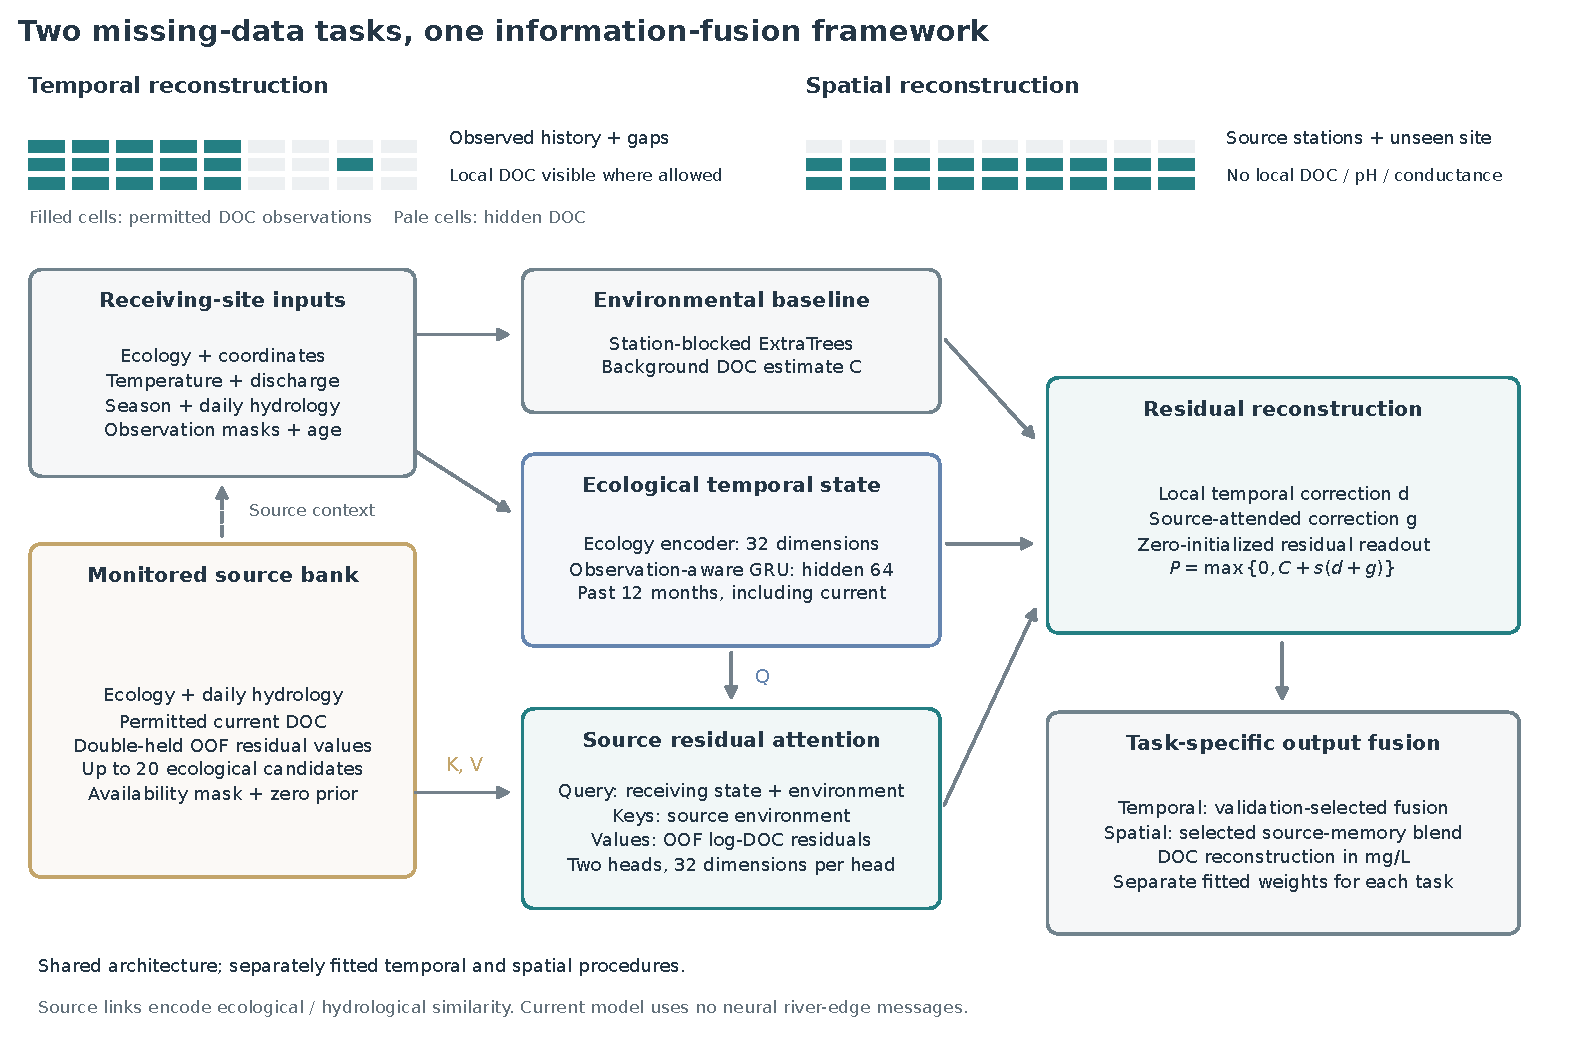
\includegraphics[width=\linewidth]{figures/spatiotemporal_v4/fig1_framework.pdf}
\caption{\textbf{Parallel temporal and spatial DOC reconstruction.} The temporal task retains legitimate local history; the spatial task hides all receiving-site chemistry. Environmental prediction supplies $C$, recurrent state supplies local correction $d$ and source attention supplies $g$. Source keys describe ecology and hydrology, while values are double-held environmental log residuals. The reconstruction is followed by task-specific validation fusion. Source similarity links and causal monthly memory organize available information; temporal and spatial weights are fitted separately.}
\label{fig:framework}
\end{figure}

\section{Results}
\subsection{Temporal reconstruction combines dynamic prediction and concentration correction}
The complete framework achieves MAE 0.785~mg/L in unobserved periods and 0.797~mg/L in observation-assisted periods (Table~\ref{tab:results}; Figure~\ref{fig:time}). Against strong environmental trees, paired reductions are 12.51\% [8.70,15.91\%] and 14.88\% [11.86,17.61\%], with all three seeds improving. $R^2$ is approximately 0.60 in both tasks. The two tasks have different query populations and information conditions; their absolute MAEs do not measure the isolated benefit of designated observations.

Native residual predictions have MAE 0.896 and 0.935~mg/L, close to their tree references. All six complete fits select log-affine validation fusion. Concentration correction therefore contributes substantially to the complete temporal result. The current source-attention increment over the previous complete temporal procedure is 0.107\% [0.011,0.199\%] in unobserved periods and 0.086\% [$-0.013$,0.188\%] in assisted periods. Temporal reconstruction remains effective after the source upgrade, while the new attention increment is small.

\begin{table}[!htbp]\centering\small
\caption{Unified main results with task-specific weighting. Concentration errors and bias are in mg/L. Positive bias means overprediction. Temporal values average three seed errors; geographical values average five seeds within region, then five regions equally; external values score a fixed five-member prediction mean.}
\label{tab:results}
\setlength{\tabcolsep}{4pt}
\begin{tabular}{>{\raggedright\arraybackslash}p{3.1cm}>{\raggedright\arraybackslash}p{4.1cm}rrrr}\toprule
Scenario & Procedure & MAE & RMSE & $R^2$ & Bias\\\midrule
Unobserved periods & Strong environmental trees & 0.897 & 1.326 & 0.527 & 0.452 \\
 & Previous complete method & 0.786 & 1.223 & 0.598 & 0.138 \\
 & Current complete method & 0.785 & 1.222 & 0.599 & 0.139 \\
Observation-assisted periods & Strong environmental trees & 0.936 & 1.339 & 0.509 & 0.561 \\
 & Previous complete method & 0.798 & 1.209 & 0.600 & 0.241 \\
 & Current complete method & 0.797 & 1.208 & 0.601 & 0.241 \\
Unmonitored regions & Strong environmental trees & 2.345 & 3.914 & 0.116 & -0.597 \\
 & Previous complete method & 2.282 & 3.865 & 0.131 & -0.649 \\
 & Current complete method & 2.249 & 3.842 & 0.144 & -0.721 \\
External application & Strong environmental trees & 0.841 & 1.240 & 0.084 & -0.034 \\
 & Previous complete method & 0.915 & 1.378 & -0.130 & -0.434 \\
 & Current complete method & 0.911 & 1.377 & -0.129 & -0.442 \\
\bottomrule

\end{tabular}
\end{table}

\begin{figure}[!htbp]\centering
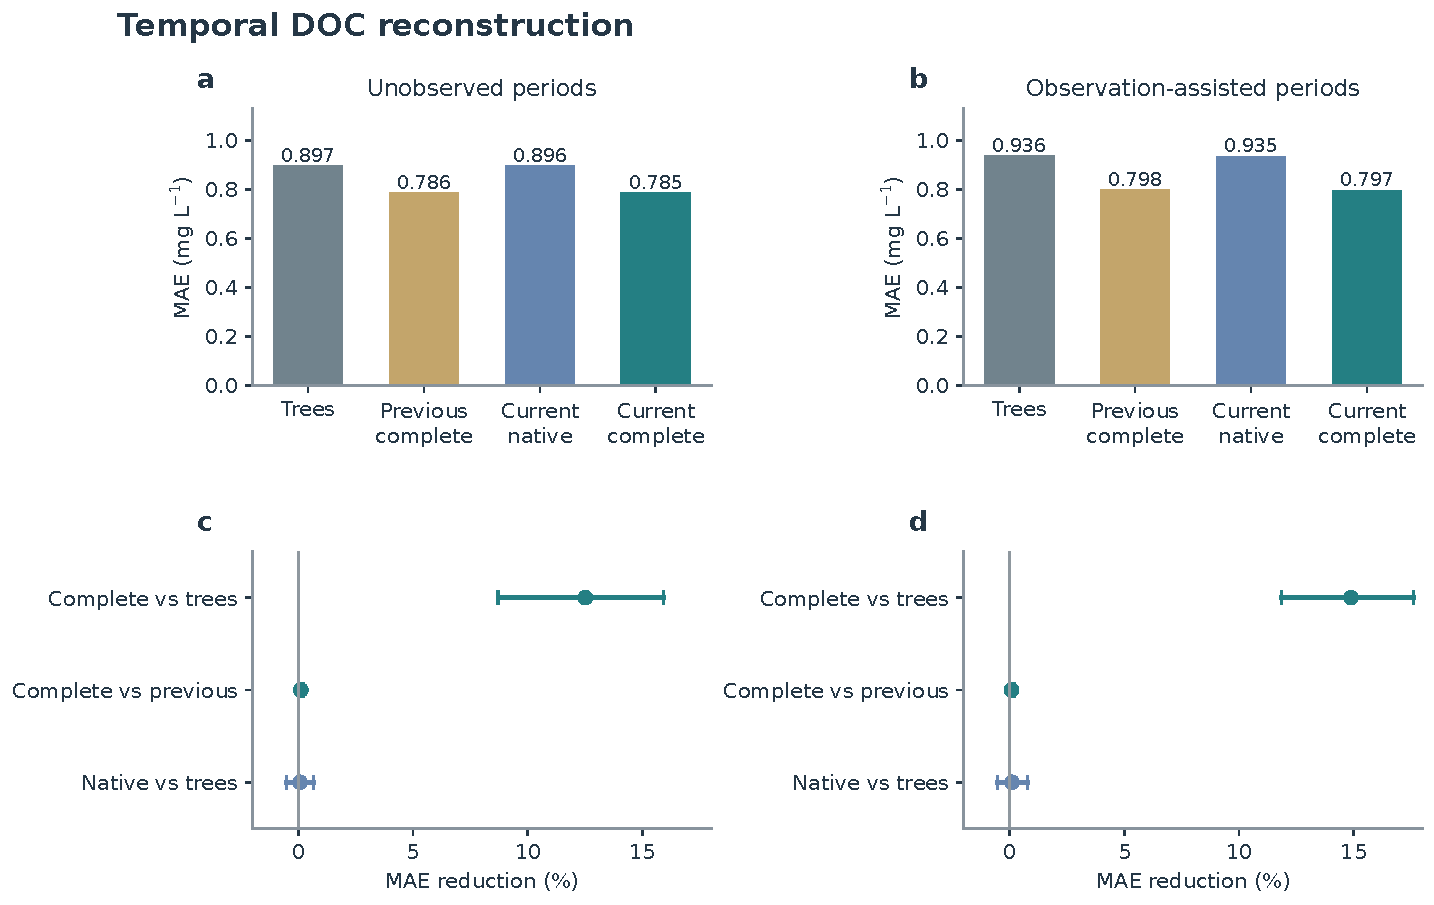
\includegraphics[width=\linewidth]{figures/spatiotemporal_v4/fig2_temporal.pdf}
\caption{\textbf{Temporal reconstruction in two observation conditions.} Top panels compare strong trees, previous complete reconstruction, current native residual prediction and current complete prediction. Bottom panels show paired MAE reductions with 95\% station-bootstrap intervals. Complete predictions include validation-selected fusion and concentration correction. Each task uses three fitted seeds; the unobserved and assisted populations contain 2,223 and 1,778 unique cells, respectively.}
\label{fig:time}
\end{figure}

\subsection{Spatial reconstruction improves across withheld regions}
Without any receiving DOC, pH or conductivity, the current complete method reaches equal-region MAE 2.249~mg/L. Strong environmental trees achieve 2.345~mg/L, and the previous complete method achieves 2.282~mg/L. Their paired reductions are 4.11\% [1.11,7.11\%] and 1.48\% [0.42,2.67\%], respectively. All five regions improve against trees, and four improve against the previous method (Figure~\ref{fig:space}).

The regions span different error scales. Current MAE ranges from 1.082~mg/L in HUC1101 to 5.583~mg/L in HUC1013. Station-equal MAE is 2.476~mg/L, reflecting a different weighting of sparse and frequently sampled sites. The lower regional MAE coexists with a more negative mean bias than the previous complete method (Table~\ref{tab:results}). The reconstruction therefore reduces absolute error while retaining a concentration-underprediction challenge.

\begin{figure}[!htbp]\centering
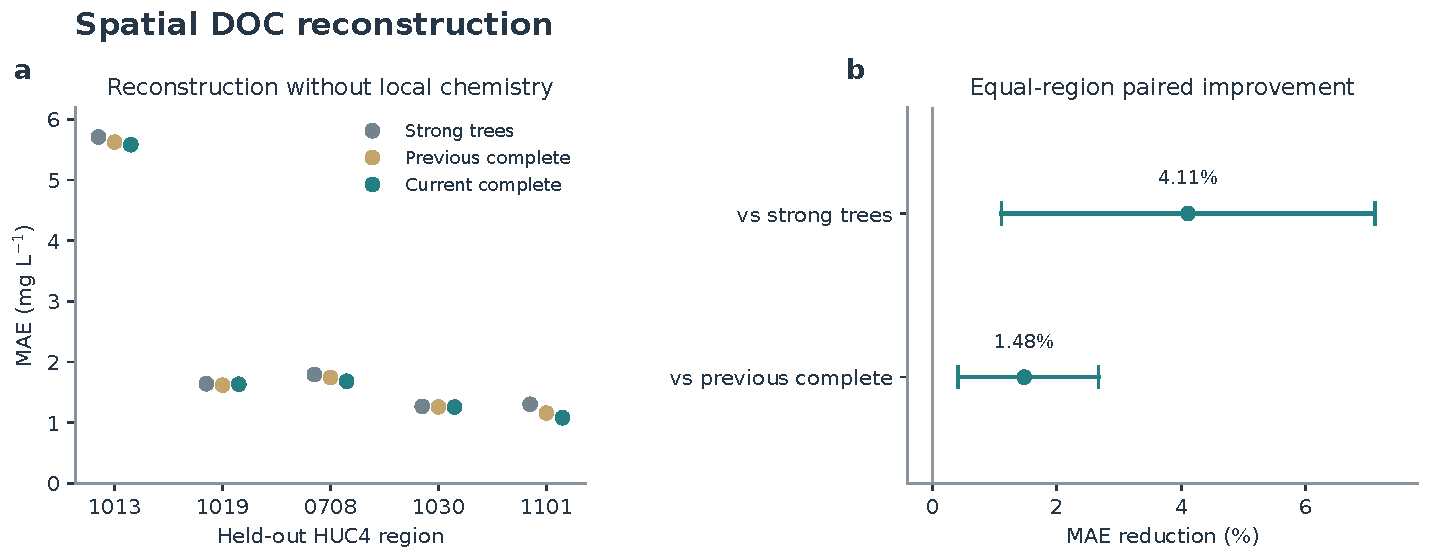
\includegraphics[width=\linewidth]{figures/spatiotemporal_v4/fig3_spatial.pdf}
\caption{\textbf{Spatial reconstruction at stations without local chemistry.} Region points are five-seed mean MAEs for the same withheld observations. Paired improvements give the five regions equal weight and use 5,000 station resamples. The evaluation contains 7,262 observed station-months at 104 stations. This is geographical withholding within ST357.}
\label{fig:space}
\end{figure}

\subsection{Current monitoring context adds information beyond seasonal source experience}
The matched source comparison holds the candidate availability and aggregate inputs fixed while substituting actual current source values for seasonal values. Actual values achieve regional MAE 2.249~mg/L, compared with 2.271 for the seasonal control: a 0.97\% reduction [0.46,1.55\%], positive in all five regions (Figure~\ref{fig:information}). This increment is present before static-memory fusion: native predictions improve 0.80\% [0.20,1.52\%] against their native seasonal counterpart.

Allowing actual current sources without an earlier-season observation also improves the matched full-source procedure by 0.78\% [0.28,1.34\%]. These comparisons support the value of contemporary monitoring context and its availability. The 4.11\% complete-method advantage against trees includes the other retained residual-learning and fusion components. Wider candidate pools and additional source-state keys did not improve their development comparisons and are summarized in Supplementary Material.

\begin{figure}[!htbp]\centering
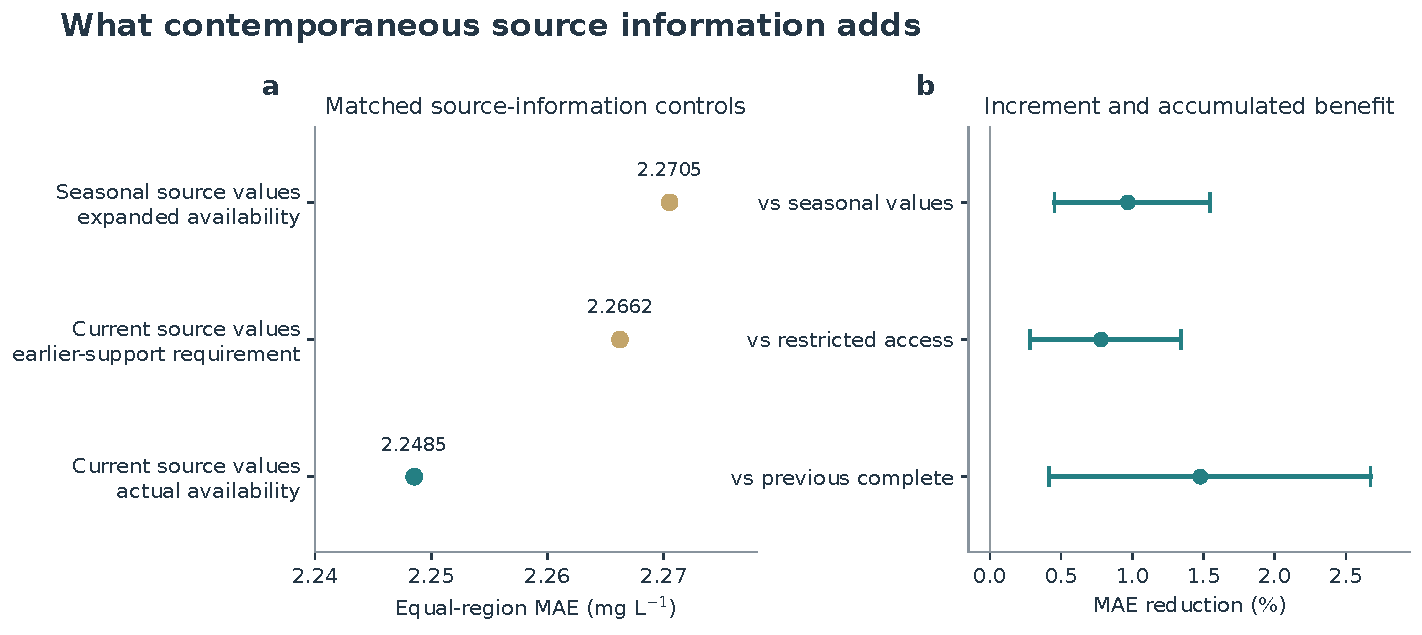
\includegraphics[width=\linewidth]{figures/spatiotemporal_v4/fig4_information.pdf}
\caption{\textbf{Matched evidence for source information.} The left panel uses a focused MAE axis to resolve differences among seasonal values, current values requiring earlier support, and all permitted current values. The seasonal comparison preserves expanded source availability and the same aggregate inputs. The right panel reports isolated current-value and access increments alongside the accumulated difference from the previous complete method; bounds are 95\% paired station-bootstrap intervals.}
\label{fig:information}
\end{figure}

\subsection{External application and sparse local observations}
The fixed five-member model achieves external MAE 0.911~mg/L, compared with 0.915 for the previous release and 0.841 for strong trees (Figure~\ref{fig:external}). Its incremental reduction over the previous release is 0.48\% [$-0.39$,1.56\%]. RMSE is 1.377~mg/L and $R^2=-0.129$, whereas trees achieve 1.240~mg/L and $R^2=0.084$. The tree reference retains the lower primary error in this basin. Current station-equal MAE is 0.821~mg/L, compared with 0.905 for trees, illustrating how unequal record lengths change the weighting of station performance.

Five designated support dates per eligible station are excluded from the query at every support count. The current model's fixed-query MAE at zero, one, three and five observations is 0.925, 0.925, 0.829 and 0.746~mg/L. Five observations reduce error by 19.35\% relative to its own fixed-query zero-observation prediction. This station-level adjustment is complementary to source-only reconstruction. Source validation selects zero adjustment for a single observation. Because support dates may follow query dates, this adaptation concerns retrospective reconstruction.

\begin{figure}[!htbp]\centering
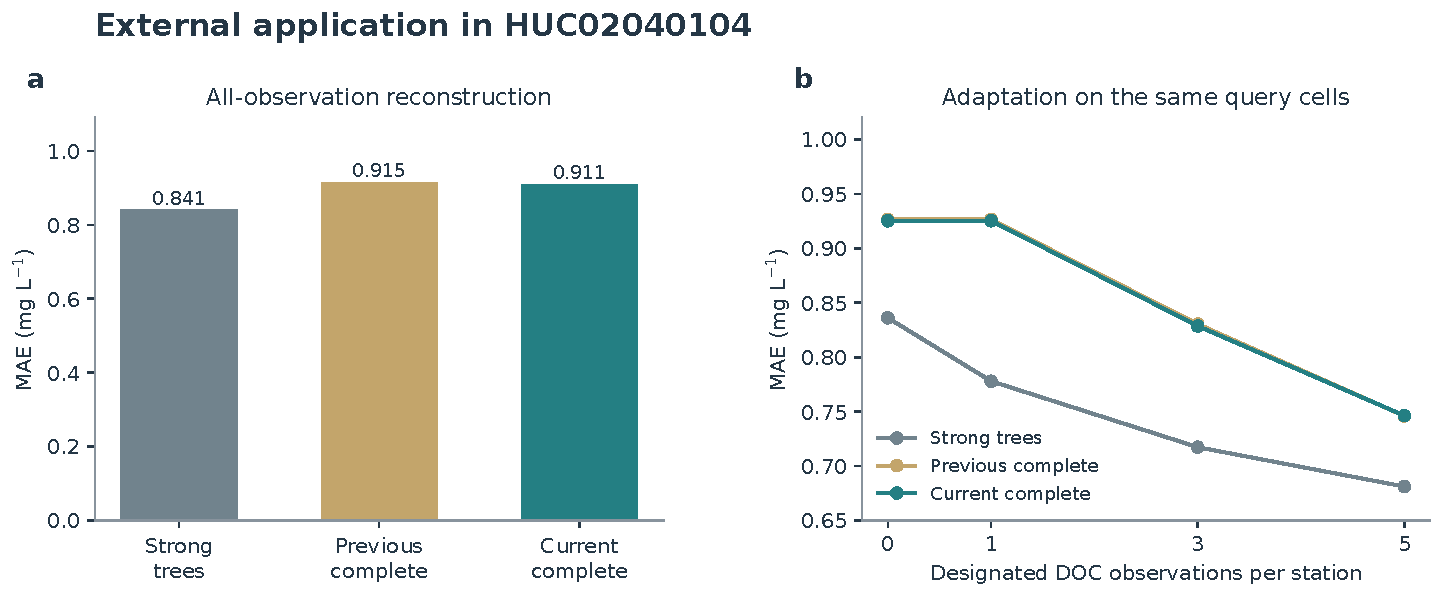
\includegraphics[width=\linewidth]{figures/spatiotemporal_v4/fig5_external.pdf}
\caption{\textbf{Fixed external application and adaptation.} The primary result scores all 6,514 observed cells at 130 external stations. The adaptation curve scores a separate set of 5,864 cells, excluding every designated support date at all support counts. All three procedures use the same populations within each panel. This basin was inspected for an earlier version; the current fixed model receives no external DOC calibration at zero support.}
\label{fig:external}
\end{figure}

\FloatBarrier
\section{Discussion}
\subsection{Complementary information under temporal and spatial missingness}
The framework gives each information source a defined role. Environmental prediction describes the catchment background, recurrent state represents time-varying conditions, and source attention selects contemporary concentration deviations from other stations. Temporal gaps can retain a local reference, whereas new stations depend more strongly on transferable environmental and source information. Treating these conditions explicitly explains why the same framework benefits from different fitted fusion policies.

The main results show that a complete spatiotemporal procedure can improve reconstruction in both time and withheld geographical regions. The matched experiments also clarify the strength of the individual evidence. Temporal improvement includes substantial concentration correction; current source observations provide a smaller, reproducible regional increment. This decomposition makes the contribution of the framework more informative than a single best-error comparison. It also preserves the environmental model as an effective reference when source or local information is weak.

Station-blocked training helps represent the information available at an unmonitored location. Double-held donor references further separate a receiving site's targets from its experience bank. The field setting itself remains observational, with correlated geography and historical development exposure; geographical blocks provide a more demanding evaluation than unrestricted random rows \citep{roberts2017}. The present source relation is ecological and hydrological similarity. The mechanism can be extended with river connectivity when that relation supplies additional information, as examined in the supplementary river-message studies.

\subsection{Concentration regimes, monitoring effort and reconstruction quality}
The external basin exposes a concentration-regime boundary: the current model's mean bias is $-0.442$~mg/L, compared with $-0.034$ for strong trees. Source experience and learned correction do not automatically transfer with the same effectiveness to every basin. Source-validation environmental and hydrological strata help locate these differences, while the discrepancy between cell-weighted and station-equal errors shows the influence of unequal monitoring intensity.

A few local measurements can help establish a receiving station's concentration reference. The 19.35\% external fixed-query improvement demonstrates this opportunity, but it is obtained by an output adjustment rather than by updating the recurrent dynamics. Upper-decile DOC groups are small in the time tasks and external case. Supplementary error and coverage tables therefore report their sample counts together with performance.

Empirical intervals also illustrate a practical trade-off. The external current model has 83.27\% coverage with median width 2.737~mg/L, compared with 92.51\% and 3.537~mg/L for trees. These intervals use source validation that also selects the model. Their coverage and width jointly describe reconstruction uncertainty; prior ranking analyses provide additional diagnostics without a monitoring-design claim.

\subsection{Future research}
The first priority is to represent concentration-regime differences more effectively while preserving the strong environmental reference. Further independently selected basins and source-role development can determine which environmental states benefit from neural correction and which require stronger adaptation. Local observations could condition recurrent state updates as well as the current concentration adjustment.

The second priority is event-sensitive DOC reconstruction. Higher-frequency chemistry paired with rainfall, discharge and incoming branch concentrations would allow the model to learn peak timing, magnitude and persistence. Current monthly records support record reconstruction but provide limited information about within-month carbon transport.

The third priority is integrating real river relationships with the existing spatial information branch. The completed structure studies identify branch organization as a candidate source of DOC-level information, while current river-message experiments provide small development gains. Geometry and transport states can enrich the framework when supported by synchronized observations. A broad network shape alone does not yet determine a stable DOC ordering. These findings are retained as a separate research archive and concise supplementary comparison.

Finally, uncertainty estimation should adapt to distribution shifts without relying on excessive interval widening. Joint treatment of concentration and discharge uncertainty would be needed to extend this concentration reconstruction to river carbon-load estimation.

\section{Conclusion}
We developed an observation-aware framework that combines environmental prediction, temporal memory and monitored source-station information to reconstruct sparse river DOC. Parallel temporal and spatial experiments achieve MAE 0.785/0.797~mg/L and 2.249~mg/L, respectively. Complete-method reductions against strong trees are 12.51/14.88\% in the temporal tasks and 4.11\% across five withheld regions. Temporal fusion contributes substantially, and matched current source observations provide a separate 0.97\% regional increment over seasonal information. External application retains a strong tree-model comparison and shows how five local observations can reduce fixed-query error by 19.35\%. The study provides a coherent basis for DOC record reconstruction and for further work on concentration transfer, high-DOC dynamics and river-specific spatial information.

\section*{Data, code and supplementary material}
The consolidated evidence table, five core figures and separate Supplementary Material are generated from saved versioned predictions. No model was fitted or selected during manuscript consolidation. Source configurations, masks, prediction sidecars, reference snapshots and component products remain in their original experiment directories. The companion supplement records task/model mappings, detailed results, uncertainty, environmental strata and archived explorations. Model fitting, prediction, component prediction and saved-state restoration retain the existing interfaces. A permanent public release identifier has not yet been assigned.

\begin{thebibliography}{99}
\bibitem{yang2017}Yang, Q., Zhang, X., Xu, X., and Asrar, G.~R. (2017). An analysis of terrestrial and aquatic environmental controls of riverine dissolved organic carbon in the conterminous United States. \emph{Water}, 9, 383. \url{https://doi.org/10.3390/w9060383}.
\bibitem{sterle2024}Sterle, G., Perdrial, J., Kincaid, D.~W., et al. (2024). CAMELS-Chem: augmenting CAMELS (Catchment Attributes and Meteorology for Large-sample Studies) with atmospheric and stream water chemistry data. \emph{Hydrology and Earth System Sciences}, 28, 611--630. \url{https://doi.org/10.5194/hess-28-611-2024}.
\bibitem{verhoef2006}Ver Hoef, J.~M., Peterson, E., and Theobald, D. (2006). Spatial statistical models that use flow and stream distance. \emph{Environmental and Ecological Statistics}, 13, 449--464. \url{https://doi.org/10.1007/s10651-006-0022-8}.
\bibitem{breiman2001}Breiman, L. (2001). Random forests. \emph{Machine Learning}, 45, 5--32. \url{https://doi.org/10.1023/A:1010933404324}.
\bibitem{geurts2006}Geurts, P., Ernst, D., and Wehenkel, L. (2006). Extremely randomized trees. \emph{Machine Learning}, 63, 3--42. \url{https://doi.org/10.1007/s10994-006-6226-1}.
\bibitem{cini2022}Cini, A., Marisca, I., and Alippi, C. (2022). Filling the G\_ap\_s: multivariate time series imputation by graph neural networks. \emph{ICLR}. \url{https://arxiv.org/abs/2108.00298}.
\bibitem{che2018}Che, Z., Purushotham, S., Cho, K., Sontag, D., and Liu, Y. (2018). Recurrent neural networks for multivariate time series with missing values. \emph{Scientific Reports}, 8, 6085. \url{https://doi.org/10.1038/s41598-018-24271-9}.
\bibitem{tian2025}Tian, S., Sha, A., Luo, Y., et al. (2025). A novel framework for river organic carbon retrieval through satellite data and machine learning. \emph{ISPRS Journal of Photogrammetry and Remote Sensing}, 221, 109--123. \url{https://doi.org/10.1016/j.isprsjprs.2025.01.028}.
\bibitem{roberts2017}Roberts, D.~R., Bahn, V., Ciuti, S., et al. (2017). Cross-validation strategies for data with temporal, spatial, hierarchical, or phylogenetic structure. \emph{Ecography}, 40, 913--929. \url{https://doi.org/10.1111/ecog.02881}.
\end{thebibliography}
\end{document}
